\documentclass[12pt,a4paper]{article}
\usepackage{fontspec}
\XeTeXlinebreaklocale "th"
\XeTeXlinebreakskip=0pt plus 1pt
\defaultfontfeatures{Ligatures=TeX}
\setmainfont[Path={fonts/TH Sarabun PSK V-1/TH Sarabun PSK V-1/},Extension=.ttf,UprightFont={*},BoldFont={* Bold},ItalicFont={* Italic},BoldItalicFont={* BoldItalic}]{THSarabun}
\setmonofont{Latin Modern Mono}
\usepackage{graphicx,amsmath,amssymb,float,caption,xcolor,hyperref,fancyhdr,tikz}
\usetikzlibrary{arrows.meta,positioning,calc}
\usepackage{geometry,booktabs,array,tabularx}
\geometry{margin=1in}
\setlength{\headheight}{19pt}
\pagestyle{fancy}\fancyhf{}\lhead{IEEE 14 บัส: 1 SG + 4 IBR, AGSI++}\rhead{\thepage}
\hypersetup{colorlinks=true,linkcolor=blue,urlcolor=blue}
\renewcommand{\arraystretch}{1.15}
\renewcommand{\abstractname}{บทคัดย่อ}
\renewcommand{\contentsname}{สารบัญ}
\renewcommand{\figurename}{รูปที่}
\renewcommand{\tablename}{ตารางที่}
\title{\textbf{การสลับโหมด GFL$\leftrightarrow$GFM บน IEEE 14 บัสด้วย AGSI++}\\
\large 1 SG + 4 IBR: กลไกสลับ ผลที่พิสูจน์ได้ และข้อจำกัดของแบบจำลอง}
\date{4 สิงหาคม 2569}
\begin{document}
\maketitle

\begin{abstract}
รายงานนี้เปลี่ยนเฉพาะข้อมูล case พารามิเตอร์อุปกรณ์ และลำดับเหตุการณ์ตาม
\path{docs/text/EECON49_[Nui].pdf} แต่ยังใช้ AGSI++ ของโครงการเป็นตัวตัดสินโหมด
โดยเพิ่ม grid-reference availability (GRA) เป็นพจน์ที่เจ็ดและเฉลี่ยใหม่ด้วยน้ำหนัก $1/7$ เท่ากัน
SG ใช้ operational EMF6/Kundur หก state ส่วน IBR ใช้ full-state GFL/GFM ที่มี filter,
DC-link, PI controller, delay และ current limit ตามค่าที่เอกสารให้ ผลที่ยืนยันได้คือจุดทำงานเป็น
equilibrium, วงควบคุมกระแสมี negative feedback ถูกทิศ, IBR สลับตาม local index/timer ของตนเอง
และ gate แบบย่อสามารถคืน ideal SG reference แล้วพา IBR1--IBR4 กลับ GFL ได้ครบ
อย่างไรก็ตาม chronology 160~s ยังหยุดแบบ fail-closed ที่ 36.040~s หลัง SG trip เพราะเอกสารไม่ให้
กฎ $I_{dc}$, active-power dispatch/energy reserve และการประสานหลาย GFM อย่างครบถ้วน
จึงไม่อ้างว่าจำลองผล 145~s ของ paper ได้ตรงทั้งหมด และไม่เติม noise หรือจูนค่าเพื่อทำให้กราฟดูสำเร็จ
\end{abstract}
\tableofcontents
\newpage

\section{คำตอบตรงตาม feedback}
\begin{tabularx}{\textwidth}{p{0.28\textwidth}X}
\toprule คำถาม & คำตอบจากโค้ดและผลจำลอง \\ \midrule
รู้ได้อย่างไรว่า IBR อยู่โหมดใด & อ่านค่า committed mode ของแต่ละอุปกรณ์โดยตรง: 0=GFL, 1=GFM ไม่อนุมานจากกราฟ $P$ หรือ $V$ \\
สลับด้วยวิธีใด & binary hybrid state machine; เงื่อนไขเป็น AGSI++ ร่วมกับ hysteresis และ dwell timer แยก IBR \\
ใช้เกณฑ์อะไร & GFL$\to$GFM เมื่อ $\mathrm{AGSI}^{++}_i\ge\Gamma_{on}$ ต่อเนื่องครบ $T_{d,on}$; GFM$\to$GFL เมื่อ index ต่ำกว่า $\Gamma_{off}$, มี grid reference และครบ $T_{d,off}$ \\
สลับพร้อมกันหรือไม่ & ไม่บังคับพร้อมกัน ผล full-state ล่าสุด IBR1--2 สลับที่ 20.130~s และ IBR3--4 ที่ 20.150~s เพราะ index/timer ต่างกัน \\
ตัวไหนเป็น slack bus & ระหว่าง island ไม่มี IBR ใดเป็น algebraic PF slack; IBR1 เป็น reference leader ที่เลือกตามลำดับเพื่อประสานมุม/ความถี่เท่านั้น ทุก IBR ยังฉีดกระแสผ่าน full KCL \\
กลับ GFL อย่างไร & การกลับตาม index เป็น local decision; ส่วน gate ตอน SG reclose ใช้ coordinated SG-reference handback ซึ่งเป็น override ที่ประกาศชัดและแยกจาก AGSI \\
\bottomrule
\end{tabularx}

\section{ขอบเขต case และที่มาของค่า}
ระบบใช้ $S_{base}=100$~MVA, $f_0=60$~Hz, SG ที่บัส 1 และ IBR1--IBR4 ที่บัส 2, 3, 6, 8
ตามรูปเครือข่ายของ EECON49 ค่า apparent-power ที่อ่านได้จากรูปคือ 36.31, 33.02, 50.86 และ
30.64~MVA การแยกเป็น $P/Q$ ใช้มุมกำลังร่วมของ case และระบุเป็น \texttt{PROJECT\_DERIVED}
เพราะ paper ไม่เผยแพร่คู่ $P/Q$ แยกกัน ค่าพารามิเตอร์อุปกรณ์เป็น \texttt{SOURCE\_DEFINED};
การแมปบัสและโหลดเป็น \texttt{CASE\_DEFINED}; AGSI++ และ state machine เป็นของโครงการ

\begin{figure}[H]\centering
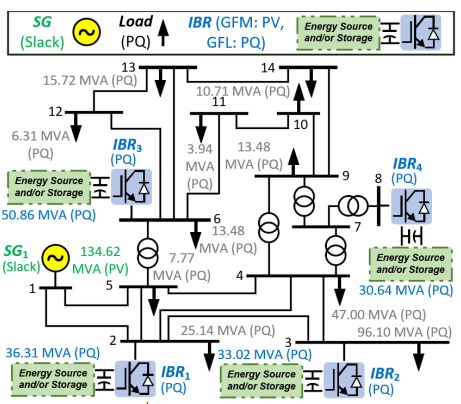
\includegraphics[width=5.90in]{figures/switch_ieee14/ieee14_oneline.png}
\caption{โครงข่ายที่ใช้จริง: SG บัส 1 และ IBR1--IBR4 ที่บัส 2, 3, 6, 8}
\end{figure}

\section{AGSI++ และความหมายตัวแปรทุกตัว}
\begin{align}
J_V&=\frac{|V-V_{ref}|}{0.10},&
J_f&=\frac{|f-60|}{0.50},&
J_R&=\frac{|\mathrm{d}f/\mathrm{d}t|}{1.0},\\
J_P&=\frac{|P_{ref}-P|}{0.20},&
J_{SCR}&=\max\left(0,\frac{3}{SCR}-1\right),&
J_{lock}&=\frac{|v_q|}{0.10},\\
J_{GRA}&=1-GRA,
\end{align}
\begin{equation}
\mathrm{AGSI}^{++}_i=\frac{J_V+J_f+J_R+J_P+J_{SCR}+J_{lock}+J_{GRA}}{7}.
\end{equation}

\noindent\begin{tabularx}{\textwidth}{@{}p{0.18\textwidth}X@{}}
\toprule สัญลักษณ์ & ความหมาย หน่วย และวิธีตีความ \\ \midrule
$V,V_{ref}$ & ขนาดแรงดัน PCC และค่าอ้างอิง หน่วย pu; $J_V$ สูงเมื่อแรงดันเบี่ยงจากค่าที่กำหนด \\
$f$ & ความถี่ Hz จาก PLL ใน GFL หรือ virtual rotor ใน GFM; 60 คือ nominal frequency \\
$\mathrm{d}f/\mathrm{d}t$ & RoCoF หน่วย Hz/s จาก accepted time samples; ตัวหาร 1.0 คือฐาน normalization \\
$P,P_{ref}$ & กำลังจริงที่ฉีดและ setpoint บนฐานระบบ หน่วย pu; $J_P$ วัด tracking error \\
$SCR$ & short-circuit ratio เชิงวินิจฉัย; ถ้า $SCR\ge3$ พจน์นี้เป็นศูนย์ ถ้าต่ำกว่า 3 stress จะเพิ่ม \\
$v_q$ & แรงดันแกน q ในกรอบ PLL หน่วย pu; ถ้าไม่ใกล้ศูนย์แสดงว่า PLL ยังจัดแนวไม่ดี \\
$GRA$ & grid-reference availability: 1 เมื่อ SG online หรือมี committed GFM reference; มิฉะนั้น 0 \\
$J_{GRA}$ & missing-reference stress: 0 เมื่อมี reference และ 1 เมื่อไม่มี \\
$i$ & หมายเลข IBR; แต่ละตัวคำนวณ index และ timer แยกกัน \\
$\Gamma_{on/off}$ & hysteresis thresholds เท่ากับ 0.65 และ 0.35 \\
$T_{d,on/off}$ & dwell time เท่ากับ 0.10~s และ 1.00~s \\
\bottomrule
\end{tabularx}

พจน์ย่อยไม่ถูก clip ให้อยู่ใน $[0,1]$ จึงเป็นไปได้ที่ AGSI++ สูงกว่า 1 และ GRA เป็นเพียง
หนึ่งพจน์น้ำหนัก $1/7$ ไม่ใช่ hard switch เมื่อ index แตะ threshold timer จะเริ่มนับ;
ถ้าหลุดเงื่อนไขก่อนครบ dwell timer ถูกยกเลิก ดังนั้นการ ``ชนเส้น'' ชั่วคราวยังไม่เท่ากับการ commit

\section{State machine: index-driven กับ coordinated handback}
\begin{figure}[H]\centering
\begin{tikzpicture}[node distance=4.5cm,>=Latex]
\node[draw,rounded corners,minimum width=3cm,minimum height=1.2cm] (a) {GFL (mode=0)};
\node[draw,rounded corners,minimum width=3cm,minimum height=1.2cm,right=of a] (b) {GFM (mode=1)};
\draw[->,thick,bend left=18] (a) to node[above,align=center] {$\mathrm{AGSI}^{++}_i\ge\Gamma_{on}$\\ครบ $T_{d,on}$} (b);
\draw[->,thick,bend left=22] (b) to node[below=5pt,align=center] {$\mathrm{AGSI}^{++}_i<\Gamma_{off}$, $GRA=1$\\ครบ $T_{d,off}$} (a);
\node[below=2.8cm of $(a)!0.5!(b)$,draw,dashed,align=center] (c)
{coordinated SG-reference handback\\คืน $P/Q$ schedule และ reinitialize GFL แบบ bumpless};
\draw[->,dashed] (c) -- (a);
\end{tikzpicture}
\caption{binary state machine พร้อม threshold, dwell และ coordinated override ที่แยกจาก index}
\end{figure}

เส้นทึบคือ \emph{index-driven switching} ปกติ ส่วนเส้นประคือ \emph{coordinated handback}
สำหรับการทดสอบ reclose: คืน ideal voltage/angle reference ของ SG, คืน topology/dispatch และส่ง
แต่ละ IBR ผ่าน equilibrium-consistent GFL initialization การกลับพร้อมกันใน gate นี้จึงเกิดจาก
คำสั่งประสาน ไม่ใช่เพราะ AGSI ของทุกตัวตัดเส้นพร้อมกัน

\section{แบบจำลอง dynamic ที่ใช้จริง}
\subsection{SG ลำดับหกแบบ Kundur/operational EMF6}
state คือ
\[
x_{SG}=[\delta,\Delta\omega,E'_q,E'_d,E''_q,E''_d]^T .
\]
$\delta$ คือมุมโรเตอร์ rad, $\Delta\omega$ คือ speed deviation pu, $E'$ และ $E''$ คือ transient และ
subtransient internal EMF บนแกน d/q สมการแกนกลมีรูป
\[
\dot\delta=\omega_0\Delta\omega,\qquad
2H\dot{\Delta\omega}=T_m-T_e-D\Delta\omega,
\]
และ state flux ใช้ $T'_{d0},T'_{q0},T''_{d0},T''_{q0}$, reactance และ stator current
$I_d,I_q$ ตาม operational EMF6 ใน repo โดย $T_m,E_{fd}$ ถูก solve จาก equilibrium แล้วตรึงคงที่
งานนี้จึงเพิ่มหก state ของเครื่องจริงแล้ว แต่ยังไม่ได้เพิ่ม governor, turbine, AVR, PSS,
synchronizer และ breaker transient การมี ``6 order'' อย่างเดียวจึงไม่สร้าง secondary power balance

\subsection{IBR full-state GFL/GFM}
GFL ใช้ 11 state จากบล็อกแหล่งอ้างอิงและ pad ศูนย์หนึ่ง state เพื่อให้ ABI สลับโหมดมีขนาด 12:
\[
[i_d,i_q,V_{dc},\theta_{PLL},\xi_{PLL},\xi_P,\xi_Q,\xi_{Id},\xi_{Iq},v_{cd,del},v_{cq,del},z_{pad}]^T.
\]
GFM ใช้
\[
[i_d,i_q,V_{dc},\theta,\omega,E,\xi_{Vd},\xi_{Vq},\xi_{Id},\xi_{Iq},v_{cd,del},v_{cq,del}]^T.
\]
ความหมายหลักคือ $i_d,i_q$ เป็นกระแส filter, $V_{dc}$ เป็นแรงดัน DC-link, $\theta_{PLL}$ และ
$\xi_{PLL}$ เป็น PLL, $\theta,\omega,E$ เป็น virtual angle/speed/EMF, $\xi$ เป็น integrator ของ PI
และ $v_{c*,del}$ เป็น delayed converter-voltage command พารามิเตอร์ที่ใช้คือ
$L_f=0.15$, $R_f=0.015$, $C_{dc}=0.10$, $V_{dc,ref}=1.0$, $I_{max}=1.2$,
$T_d=0.02$, $k_{p,Idq}=0.30$, $k_{i,Idq}=4.00$ รวมทั้ง gain GFL/GFM อื่นตามตาราง EECON49
วง current PI ใช้ error $i^*-i$; การใช้ $i-i^*$ จะเป็น positive feedback และถูก falsify ด้วย
fixed-bus eigenvalue test แล้ว

ข้อจำกัดสำคัญคือ paper วาด energy source/storage แต่ไม่ให้ control law ของ $I_{dc}$ โค้ดจึงปิด
energy port แบบ ideal instantaneous balance $I_{dc}=P_{ac}/V_{dc}$ เพื่อไม่ประดิษฐ์ gain ใหม่
วิธีนี้รักษา $V_{dc}$ แต่ไม่ใช่แบบจำลอง energy reserve และใช้พิสูจน์กำลังสำรองระยะยาวไม่ได้

\section{ผล Power Flow}
PF ใช้ in-house Newton--Raphson ของโครงการ ตารางต่อไปสร้างจากผล solver โดยตรง
\begin{table}[H]\centering\caption{ผล PF รายบัส (pu, ฐาน 100 MVA)}
\resizebox{\textwidth}{!}{% Generated by scripts/reporting/generate_ieee14_switch_report_figures.m.
\begin{tabular}{rrrrrrrr}\toprule
Bus & Type & $|V|$ & $\theta$ (deg) & $P_g$ & $Q_g$ & $P_L$ & $Q_L$ \\ \midrule
1 & REF & 1.06000 & +0.0000 & +2.32393 & -0.16549 & 0.00000 & 0.00000 \\ 
2 & PV & 1.04500 & -4.9826 & +0.40000 & +0.43557 & 0.21700 & 0.12700 \\ 
3 & PV & 1.01000 & -12.7251 & +0.00000 & +0.25075 & 0.94200 & 0.19000 \\ 
4 & PQ & 1.01767 & -10.3129 & +0.00000 & +0.00000 & 0.47800 & -0.03900 \\ 
5 & PQ & 1.01951 & -8.7739 & +0.00000 & +0.00000 & 0.07600 & 0.01600 \\ 
6 & PV & 1.07000 & -14.2209 & -0.00000 & +0.12731 & 0.11200 & 0.07500 \\ 
7 & PQ & 1.06152 & -13.3596 & +0.00000 & +0.00000 & 0.00000 & 0.00000 \\ 
8 & PV & 1.09000 & -13.3596 & +0.00000 & +0.17623 & 0.00000 & 0.00000 \\ 
9 & PQ & 1.05593 & -14.9385 & +0.00000 & +0.00000 & 0.29500 & 0.16600 \\ 
10 & PQ & 1.05098 & -15.0973 & +0.00000 & +0.00000 & 0.09000 & 0.05800 \\ 
11 & PQ & 1.05691 & -14.7906 & +0.00000 & +0.00000 & 0.03500 & 0.01800 \\ 
12 & PQ & 1.05519 & -15.0756 & +0.00000 & +0.00000 & 0.06100 & 0.01600 \\ 
13 & PQ & 1.05038 & -15.1563 & +0.00000 & +0.00000 & 0.13500 & 0.05800 \\ 
14 & PQ & 1.03553 & -16.0336 & +0.00000 & +0.00000 & 0.14900 & 0.05000 \\ 
\bottomrule\end{tabular}
}
\end{table}
\begin{table}[H]\centering\caption{line flow ด้าน from และ line loss (pu)}
\resizebox{\textwidth}{!}{% Generated by scripts/reporting/generate_ieee14_switch_report_figures.m.
\begin{tabular}{r@{\hspace{0.8em}}r@{\hspace{0.8em}}r@{\hspace{0.8em}}r@{\hspace{0.8em}}r@{\hspace{0.8em}}r@{\hspace{0.8em}}r}\toprule
Line & From & To & $P_{from}$ & $Q_{from}$ & $P_{loss}$ & $Q_{loss}$ \\ \midrule
1 & 1 & 2 & +0.900928 & -0.203057 & +0.014518 & -0.014696 \\
2 & 1 & 5 & +0.418019 & -0.066451 & +0.008475 & -0.019813 \\
3 & 2 & 3 & +0.464318 & -0.000621 & +0.009133 & -0.009246 \\
4 & 2 & 4 & +0.314334 & -0.079982 & +0.005358 & -0.021354 \\
5 & 2 & 5 & +0.209348 & -0.060569 & +0.002332 & -0.031219 \\
6 & 3 & 4 & -0.197092 & -0.022968 & +0.002456 & -0.007604 \\
7 & 4 & 5 & -0.447907 & +0.102332 & +0.002561 & +0.008079 \\
8 & 4 & 7 & +0.017005 & -0.115901 & +0.000000 & +0.002495 \\
9 & 4 & 9 & +0.062330 & -0.021423 & +0.000000 & +0.002062 \\
10 & 5 & 6 & +0.090091 & +0.002266 & -0.000000 & +0.001610 \\
11 & 6 & 11 & +0.130988 & +0.058687 & +0.001540 & +0.003226 \\
12 & 6 & 12 & +0.085939 & +0.026725 & +0.000784 & +0.001631 \\
13 & 6 & 13 & +0.207419 & +0.084233 & +0.002610 & +0.005140 \\
14 & 7 & 8 & -0.268840 & -0.133746 & +0.000000 & +0.013242 \\
15 & 7 & 9 & +0.285846 & +0.015351 & +0.000000 & +0.007516 \\
16 & 9 & 10 & -0.003741 & +0.022196 & +0.000013 & +0.000036 \\
17 & 9 & 14 & +0.056917 & +0.023544 & +0.000403 & +0.000857 \\
18 & 10 & 11 & -0.093754 & -0.035839 & +0.000693 & +0.001622 \\
19 & 12 & 13 & +0.024155 & +0.009094 & +0.000119 & +0.000108 \\
20 & 13 & 14 & +0.093845 & +0.030080 & +0.001359 & +0.002767 \\
\bottomrule\end{tabular}
}
\end{table}

\section{หลักฐานเวลา เหตุการณ์ index timer และโหมด}
\begin{table}[H]\centering
\caption{audit table ของ full chronology และ recovery gate}
\begin{tabularx}{\textwidth}{p{0.12\textwidth}p{0.23\textwidth}X p{0.22\textwidth}}
\toprule เวลา (s) & เหตุการณ์ & AGSI++/timer & โหมดก่อน--หลังและเหตุผล \\ \midrule
0 & no event & index ต่ำ, timer idle & ทุกตัว GFL$\to$GFL \\
20 & SG1 trip & GRA หายชั่วขณะและ on-timer เริ่มตาม local index & ยัง GFL ระหว่าง dwell \\
20.130 & local dwell ครบ & IBR1--2 ผ่านเงื่อนไขก่อน & IBR1--2 GFL$\to$GFM \\
20.150 & local dwell ครบ & IBR3--4 ผ่านเงื่อนไขถัดมา 20 ms & IBR3--4 GFL$\to$GFM \\
36.040 & long-run limit & frequency ลดถึงประมาณ 43.69 Hz และ state ออก validity domain & fail-closed; ยังไม่ถึง load/fault/line/reclose \\
1.000 (gate) & compressed SG trip & local on-timer เริ่ม & ทุกตัวเริ่มจาก GFL \\
1.120 (gate) & local dwell & IBR1--2 commit & GFL$\to$GFM \\
1.140 (gate) & local dwell & IBR3--4 commit & GFL$\to$GFM \\
3.000 (gate) & ideal SG reclose & coordinated reference handback & ทุกตัว GFM$\to$GFL พร้อมกันเพราะ override \\
4.000 (gate) & end & Newton converged, $\min|V|=1.033013$ pu & ทุกตัวคง GFL, switch count 2 ต่อตัว \\
\bottomrule
\end{tabularx}
\end{table}

\begin{figure}[H]\centering
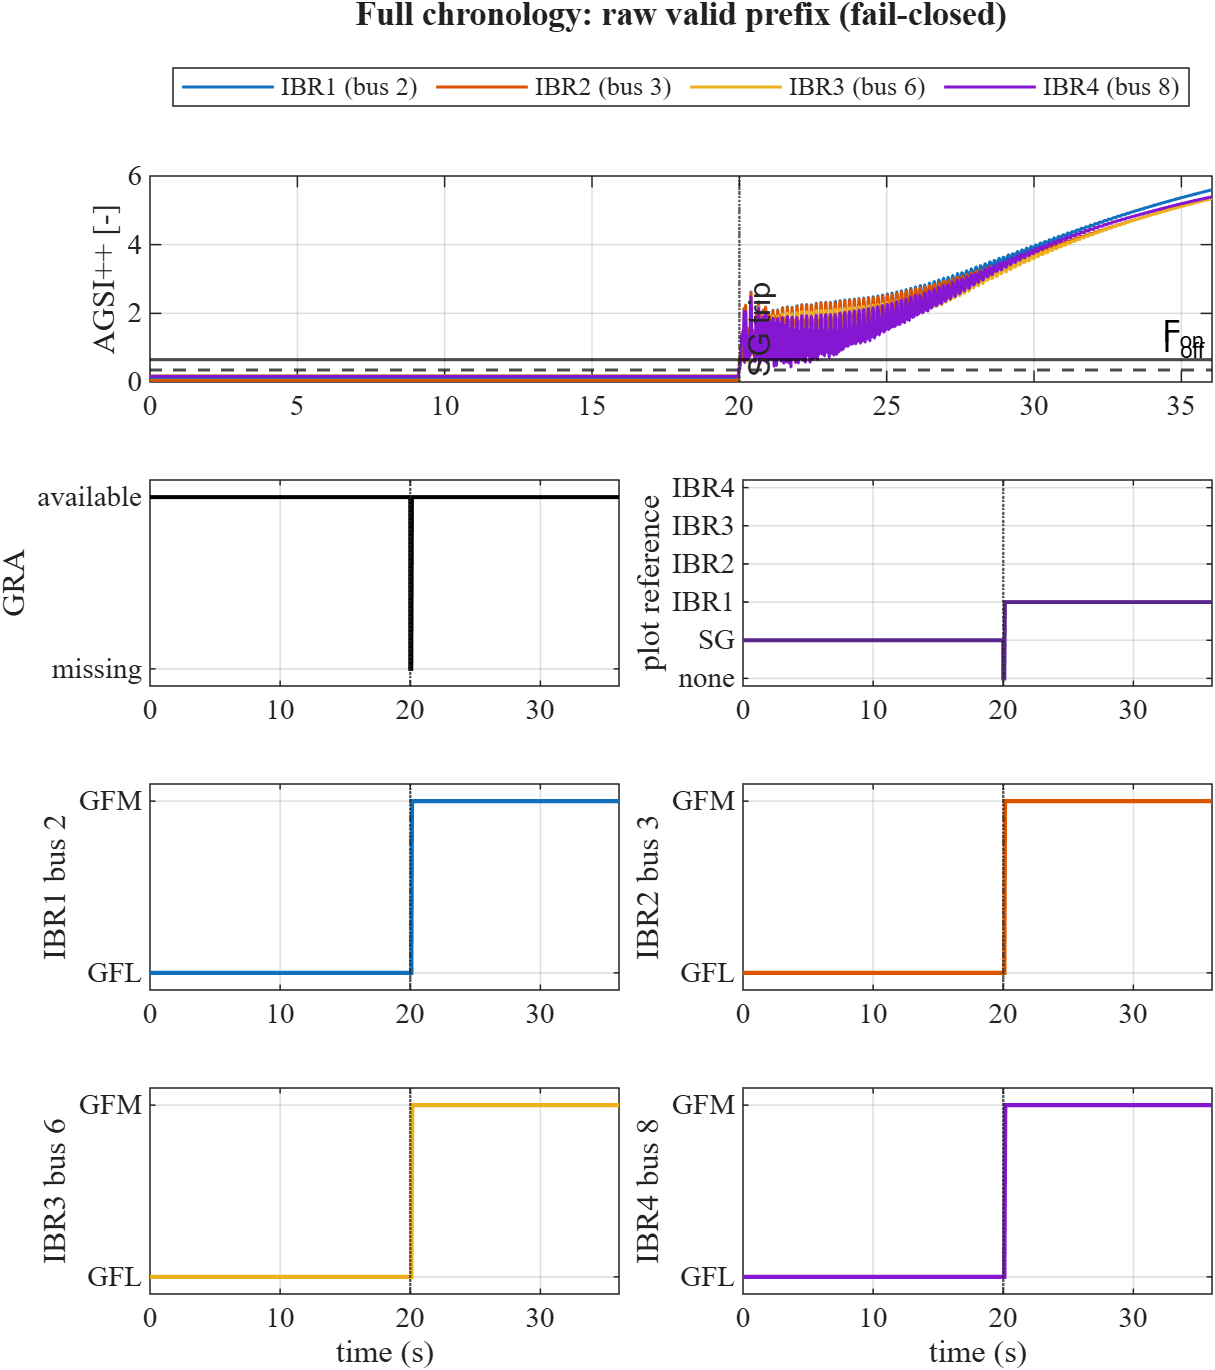
\includegraphics[width=5.90in]{figures/switch_ieee14/padiyar_switch_supervisor.png}
\caption{full chronology: AGSI++, GRA, reference และ mode timeline 0=GFL/1=GFM แยก IBR1--IBR4 ถึงจุด fail-closed}
\end{figure}
\begin{figure}[H]\centering
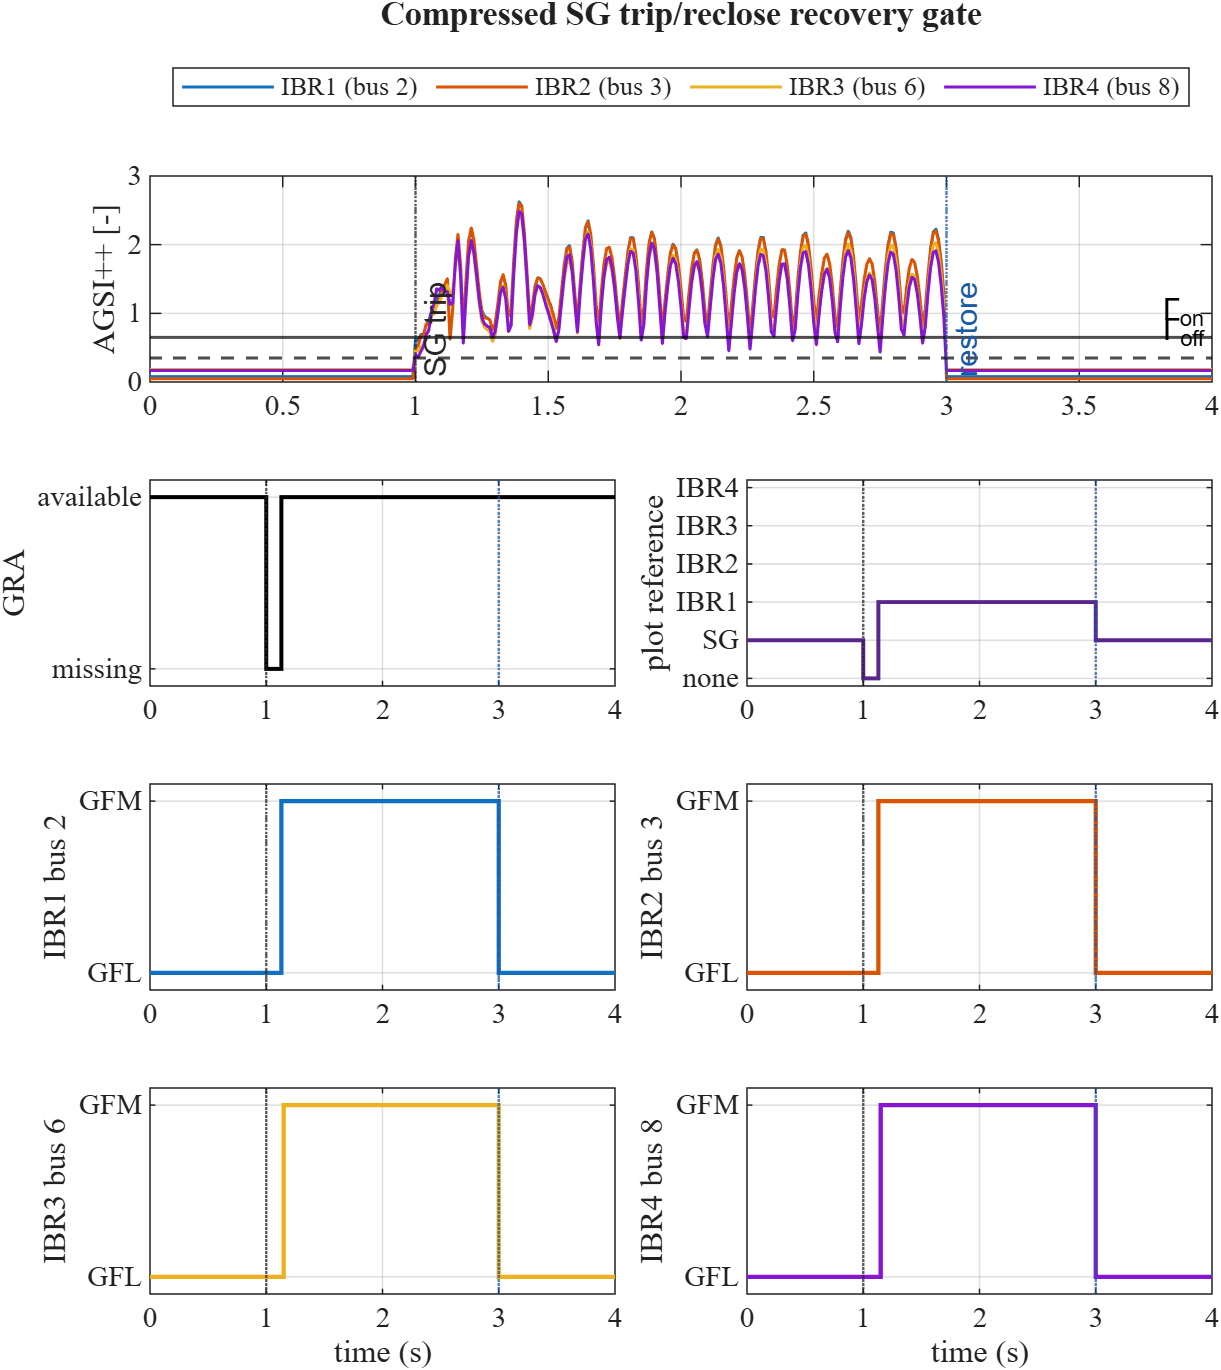
\includegraphics[width=5.90in]{figures/switch_ieee14/padiyar_switch_recovery_supervisor.png}
\caption{compressed recovery gate: timeline แสดง local GFL$\to$GFM และ coordinated GFM$\to$GFL ที่ SG reclose}
\end{figure}
\begin{figure}[H]\centering
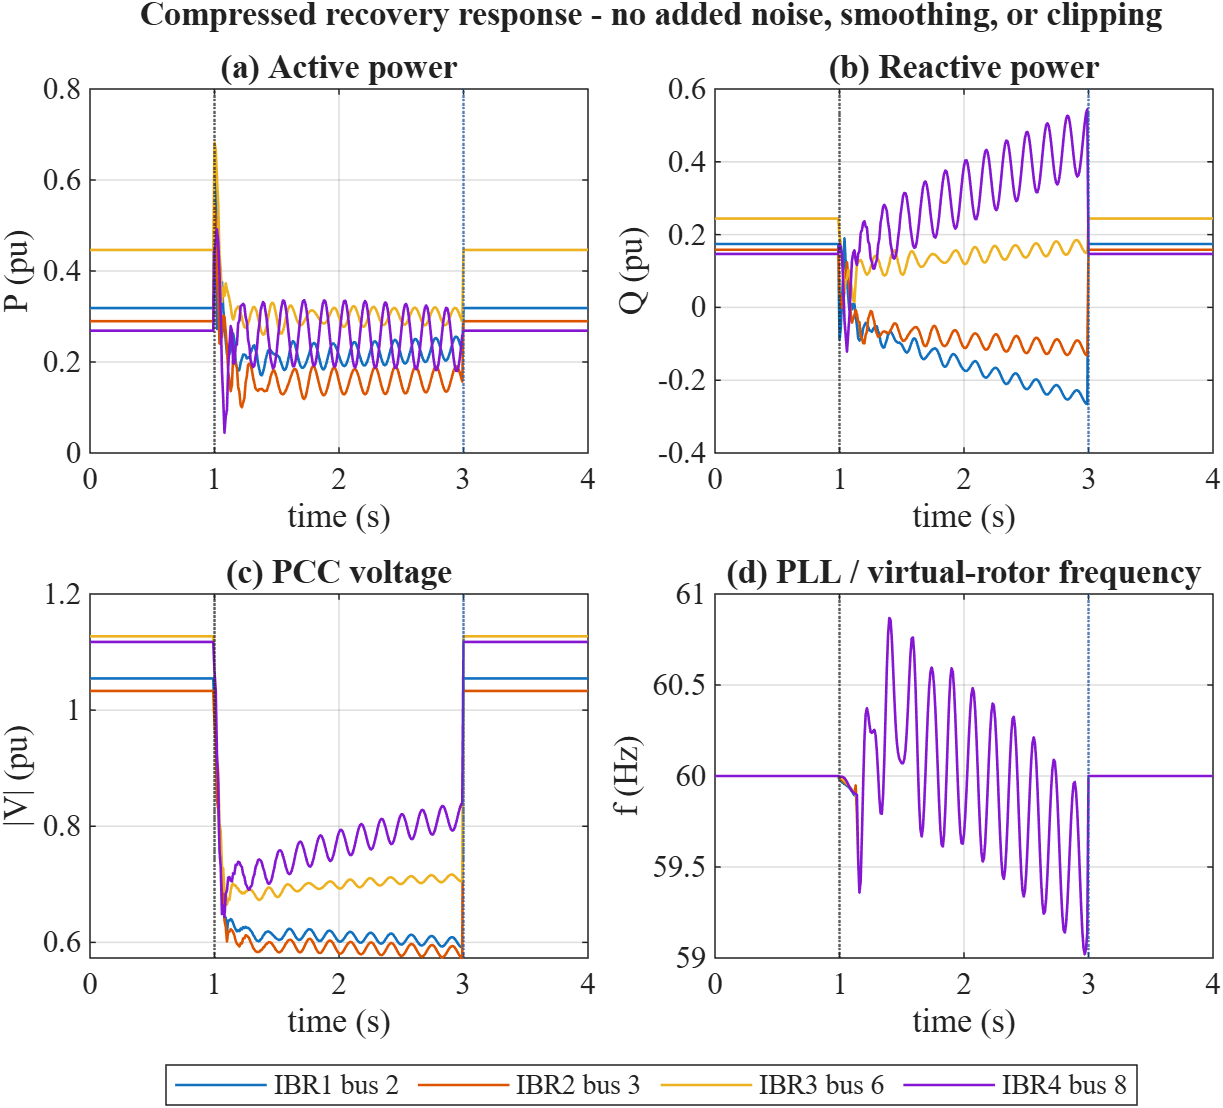
\includegraphics[width=5.90in]{figures/switch_ieee14/padiyar_switch_recovery_response.png}
\caption{ผล $P,Q,|V|,f$ ของ recovery gate จากข้อมูลดิบ ไม่มี noise, smoothing, filtering หรือ clipping}
\end{figure}

\section{สรุปหลายเหตุการณ์ที่มีหลักฐานแล้ว}
\noindent\begin{tabularx}{\textwidth}{p{0.23\textwidth}X}
\toprule เหตุการณ์ & ขอบเขตหลักฐาน \\ \midrule
no-event & full-state equilibrium residual ต่ำกว่า $10^{-9}$ และไม่มี false switch \\
fault เบา & switching-map เดิมมี ride-through เมื่อ index ไม่อยู่เหนือเส้นครบ dwell \\
fault รุนแรง & switching-map เดิมแสดง index-driven switch ได้ แต่ convergence ไม่เท่ากับ recovery \\
load step & test เดิมรองรับ +10, +30, +50\% โดยไม่สลับ; chronology EECON49 กำหนด +20\% แต่ long run ปัจจุบันล้มก่อนถึง 50~s \\
SG trip & full-state run ทำให้ IBR สลับเป็น GFM แบบ 2+2 ไม่พร้อมกันเป๊ะ \\
SG reclose & compressed ideal-slack gate ผ่านและคืน GFL ครบ; ยังไม่ใช่หลักฐาน chronology 145~s \\
line trip/reclose & event contract มีแล้ว แต่ full-state long run ยังไปไม่ถึง 110/145~s \\
\bottomrule
\end{tabularx}

\section{ทำไมเพิ่ม state แล้วจึงยังไม่เหมือน paper ทั้งหมด}
การเพิ่ม SG เป็นหก state และ IBR เป็น full-state จำเป็น เพราะกำจัดข้อจำกัด reduced-6 และทำให้
วง filter/controller/limit ปรากฏจริง แต่ยังไม่เพียงพอสำหรับ island 20--145~s หลัง SG trip
กำลังจาก SG หายไปต้องถูกชดเชยโดยกฎแบ่ง $P_{ref}$, energy reserve และ frequency restoration
ระหว่างหลาย GFM หากทุกตัวถือ setpoint เดิม ระบบมี power deficit และความถี่ลดต่อเนื่อง

ใน PDF มี block diagram และพารามิเตอร์อุปกรณ์ แต่ไม่เผยแพร่ (1) $I_{dc}$ control/energy limit,
(2) กฎเลือกและ synchronize reference ระหว่างหลาย GFM, (3) active-power sharing/secondary dispatch
หลัง SG trip และ (4) logic เปลี่ยน reference กลับ SG อย่างละเอียด การเดากฎเหล่านี้แล้วปรับจนกราฟ
เหมือน paper จะขัด numerical-integrity contract ดังนั้นผลที่ถูกต้องที่สุดตอนนี้คือ:
\begin{itemize}
\item \textbf{พิสูจน์แล้ว}: full-state equilibrium, local stability gate, local mode switching และ compressed coordinated handback;
\item \textbf{ยังไม่พิสูจน์}: trajectory เหตุการณ์เต็มถึง 160~s และ recovery ที่ 145~s;
\item \textbf{สาเหตุปัจจุบัน}: missing dispatch/energy/reference-coordination contract ไม่ใช่จำนวน state ของ SG เพียงอย่างเดียว;
\item \textbf{ไม่ทำ}: เติม noise, reset trajectory, เปลี่ยน threshold, smooth หรือ clip เพื่อสร้างผลสำเร็จเทียม
\end{itemize}

\section{การสร้างซ้ำและสถานะการตรวจสอบ}
\begin{verbatim}
pf_init_paths;
addpath(fullfile('scripts','reporting'));
generate_ieee14_switch_report_figures;
\end{verbatim}
generator ใช้ project-owned MATLAB และ $\Delta t=0.01$~s ทั้ง long diagnostic และ short recovery gate
SSSA sweep และ fault-outcome table ถูกตัดออกจากรายงานนี้เพื่อเน้น switching เท่านั้น
targeted tests ครอบคลุม full-state route/equilibrium, fixed-bus eigenvalues, coordinated handback,
legacy IEEE14 switching และ EMF6 contracts ส่วน full repository regression ไม่จำเป็นสำหรับ scope นี้
ตาม risk policy ของโครงการ

\end{document}
